\documentclass[UTF8,a4paper,11pt]{ctexart}
\usepackage[margin=2.5cm]{geometry}
\usepackage{graphicx,booktabs,array,amsmath,amssymb,float,hyperref}
\usepackage{setspace}
\setstretch{1.25}
\hypersetup{colorlinks=true,linkcolor=black,urlcolor=blue}
\graphicspath{{./}}
\title{自然语言处理作业一实验报告}
\author{姓名：强博\quad 学号：2313825}
\date{\today}
\begin{document}
\maketitle
\section{实验目的}
本实验旨在理解不同文本表示方法的基本原理，掌握新闻分类的标准实验流程，使用逻辑回归完成基于词袋和词向量的分类，并通过微调 BERT 了解预训练语言模型的使用方式。实验统一比较 Accuracy 和 Macro-F1，分析模型性能差异及类别不均衡的影响。

\section{数据集与实验设置}
\subsection{数据集}
NYT 数据集包含新闻文本 text 和类别标签 label，共 11,519 条样本，其中 business 1,429 条、politics 1,451 条、sports 8,639 条。AG News 数据集用于训练另一组 Word2Vec 词向量。NYT 按照 80\%/10\%/10\% 分层划分，随机种子设置为 42，所有分类实验使用相同划分。
\begin{table}[H]\centering\caption{NYT 数据集划分}\begin{tabular}{lrr}\toprule 数据集 & 数量 & 比例\\\midrule 训练集 & 9,215 & 80\%\\验证集 & 1,152 & 10\%\\测试集 & 1,152 & 10\%\\\bottomrule\end{tabular}\end{table}
\begin{figure}[H]\centering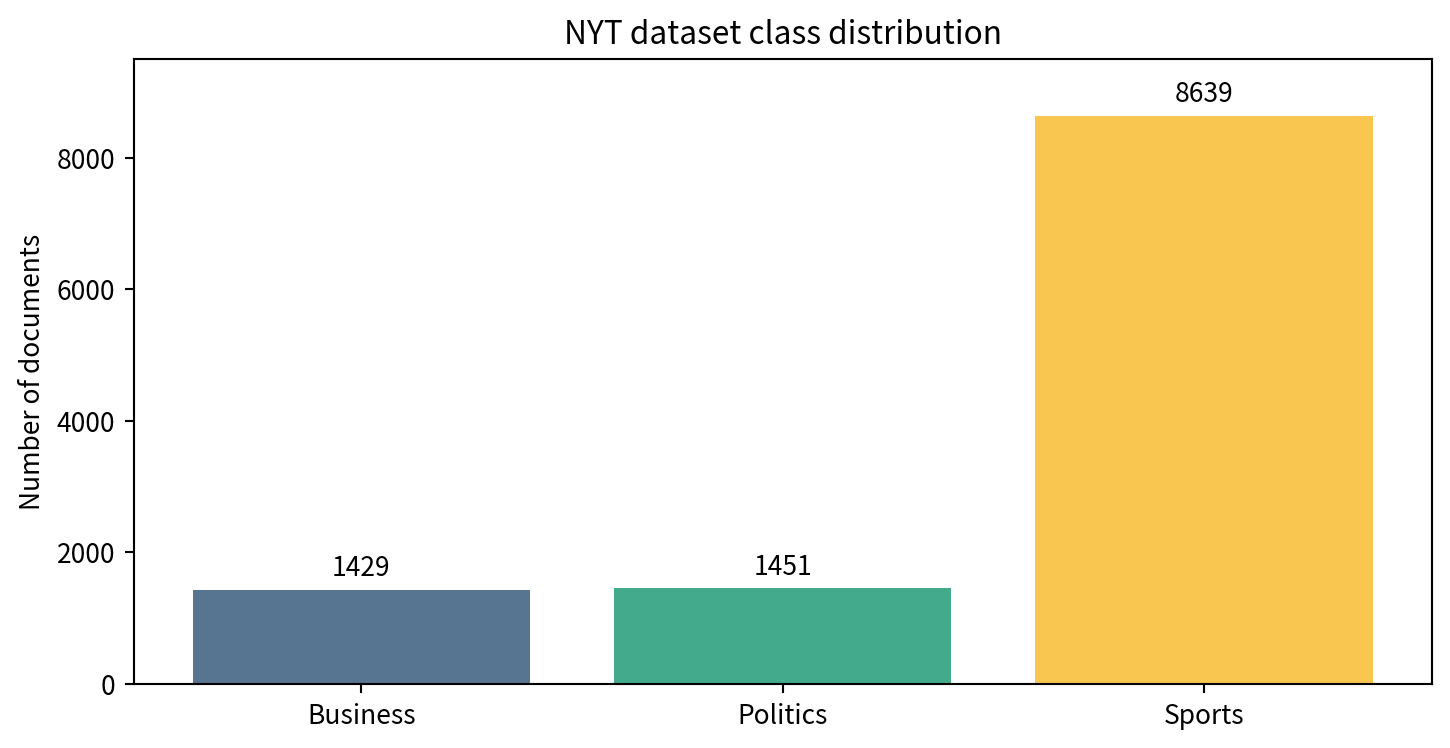
\includegraphics[width=.85\linewidth]{fig1_nyt_distribution.png}\caption{NYT 数据集类别分布}\end{figure}
体育类样本明显多于其他两类，故不能只用总体准确率衡量模型，应同时考察 Macro-F1。

\subsection{评价指标}
准确率定义为正确预测的样本数占总样本数的比例：
\begin{equation}\mathrm{Accuracy}=\frac{N_{\mathrm{correct}}}{N_{\mathrm{total}}}.\end{equation}
对类别 $i$，精确率、召回率及 F1 分别为
\begin{equation}P_i=\frac{TP_i}{TP_i+FP_i},\quad R_i=\frac{TP_i}{TP_i+FN_i},\quad F1_i=\frac{2P_iR_i}{P_i+R_i}.\end{equation}
\begin{equation}\mathrm{Macro\text{-}F1}=\frac{1}{C}\sum_{i=1}^{C}F1_i,\qquad C=3.\end{equation}
Macro-F1 为每个类别赋予相同权重，能更全面地反映不均衡数据上的分类能力。

\section{Task 1：Bag of Words 文本分类}
\subsection{方法与实现}
词袋模型将文档映射到基于训练集词表的稀疏向量空间。二值词袋（Binary BoW）只记录单词是否出现：
\begin{equation}x_i=\begin{cases}1,&w_i\text{ 在文档中出现},\\0,&\text{否则}.\end{cases}\end{equation}
词频词袋（Word Frequency BoW）则记录单词出现次数 $c_i$，得到 $\mathbf{x}=(c_1,\ldots,c_{|V|})$。两种表示均使用 Logistic Regression 训练分类器；词表只在训练集上构建，再应用于验证集和测试集，以避免数据泄漏。
\subsection{实验结果与分析}
\begin{table}[H]\centering\caption{Task 1 验证集与测试集结果}\small\begin{tabular}{lrrrr}\toprule 方法 & Val Acc & Val F1 & Test Acc & Test F1\\\midrule Binary BoW & 0.9809 & 0.9551 & 0.9887 & 0.9718\\Word Frequency BoW & \textbf{0.9835} & \textbf{0.9626} & \textbf{0.9896} & \textbf{0.9743}\\\bottomrule\end{tabular}\end{table}
两种模型均取得较高性能，说明新闻类别与词汇分布有较强关联。可以发现，词频词袋的测试集 Accuracy 和 Macro-F1 分别为 98.96\% 与 97.43\%，均略高于二值词袋，说明词语重复次数可提供额外信息。

\section{Task 2：Word Embedding 文本分类}
\subsection{方法与实现}
词向量将单词映射到低维连续空间。本任务统一采用 100 维词向量，并对文档中有有效向量的单词取平均：
\begin{equation}\mathbf{e}(d)=\frac{1}{n}\sum_{i=1}^{n}\mathbf{e}(w_i).\end{equation}
再以平均文档向量训练 Logistic Regression。比较三种表示：（1）公开预训练的 GloVe 6B 100d；（2）基于 AG News 语料训练的 Word2Vec；（3）基于 NYT 语料训练的 Word2Vec。
\subsection{实验结果与分析}
\begin{table}[H]\centering\caption{Task 2 验证集与测试集结果}\small\begin{tabular}{lrrrr}\toprule 方法 & Val Acc & Val F1 & Test Acc & Test F1\\\midrule GloVe 100d & 0.9774 & 0.9500 & \textbf{0.9852} & \textbf{0.9646}\\Word2Vec (AG News) & 0.9653 & 0.9248 & 0.9766 & 0.9416\\Word2Vec (NYT) & 0.9679 & 0.9293 & 0.9818 & 0.9542\\\bottomrule\end{tabular}\end{table}
\begin{figure}[H]\centering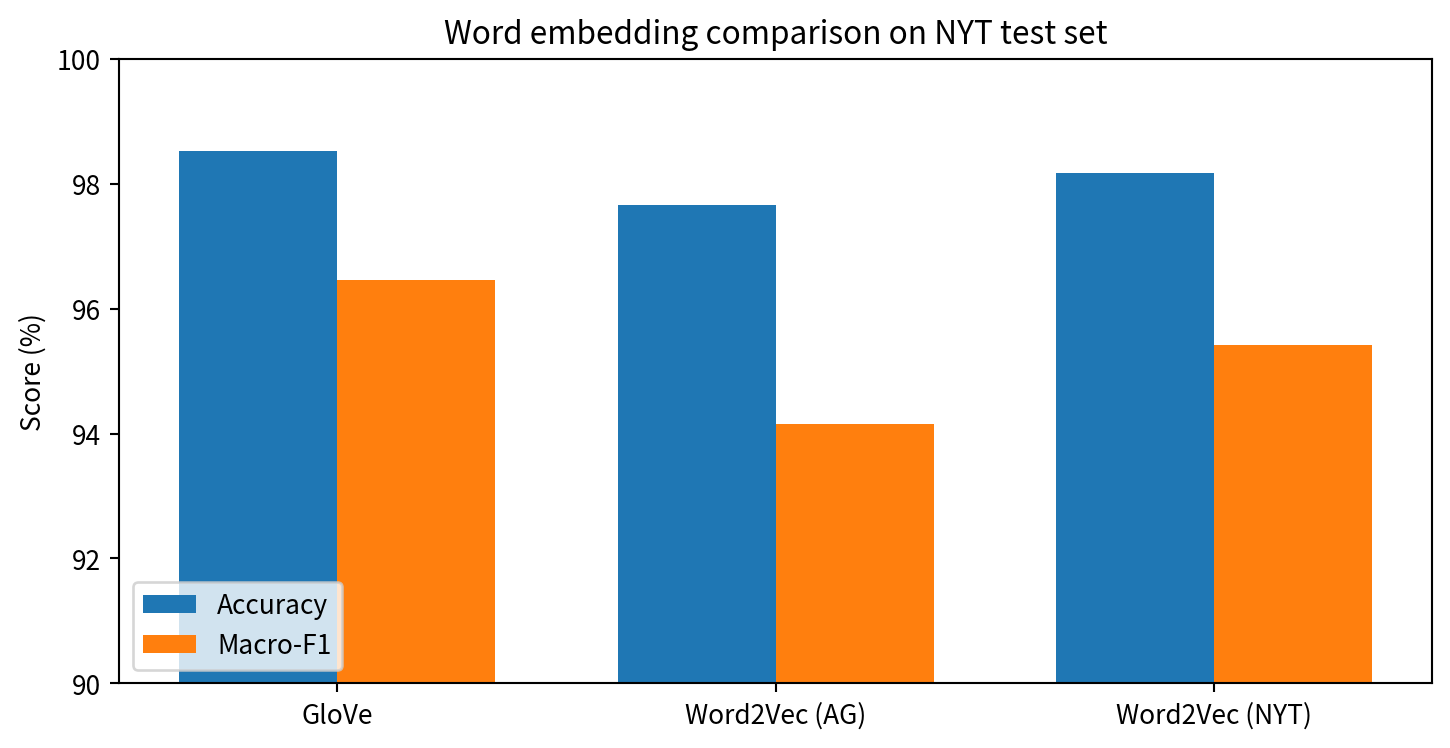
\includegraphics[width=.85\linewidth]{fig2_embeddings.png}\caption{三种词向量方案的测试集表现}\end{figure}
上述三种方法中，预训练 GloVe 表现最好，是因为其更充分的预训练语料和词汇共现信息。NYT Word2Vec 优于 AG News Word2Vec，两种方法的区别在于训练使用的语料不同，一定程度上说明训练语料与目标任务的领域匹配程度可能影响分类效果；同时Task2采用的是平均池化方法，没有办法保留词序和复杂的上下文信息。

\section{Task 3：BERT 微调分类}
\subsection{模型与训练设置}
BERT（Bidirectional Encoder Representations from Transformers）是一种基于 Transformer Encoder 的预训练语言模型。

与传统词袋模型和静态词向量不同，BERT 能够结合上下文生成动态文本表示。同一个单词在不同语境下，可以得到不同的上下文特征。

本任务使用 \texttt{google-bert/bert-base-uncased}，最大序列长度设为 64，训练 3 epochs。BERT 利用双向 Transformer 编码器产生上下文相关的表示，并通过分类头预测新闻类别。
\begin{table}[H]\centering\caption{BERT 主要训练配置}\begin{tabular}{ll}\toprule 参数 & 设置\\\midrule 预训练模型 & bert-base-uncased\\最大序列长度 & 64\\训练轮数 & 3\\学习率 & $2\times 10^{-5}$\\训练 batch size & 16\\评估 batch size & 32\\随机种子 & 42\\\bottomrule\end{tabular}\end{table}
\subsection{验证集结果}
\begin{table}[H]\centering\caption{BERT 每轮验证集性能}\begin{tabular}{lrr}\toprule Epoch & Accuracy & Macro-F1\\\midrule 1 & 0.9688 & 0.9315\\2 & \textbf{0.9766} & \textbf{0.9524}\\3 & 0.9757 & 0.9498\\\bottomrule\end{tabular}\end{table}
\begin{figure}[H]\centering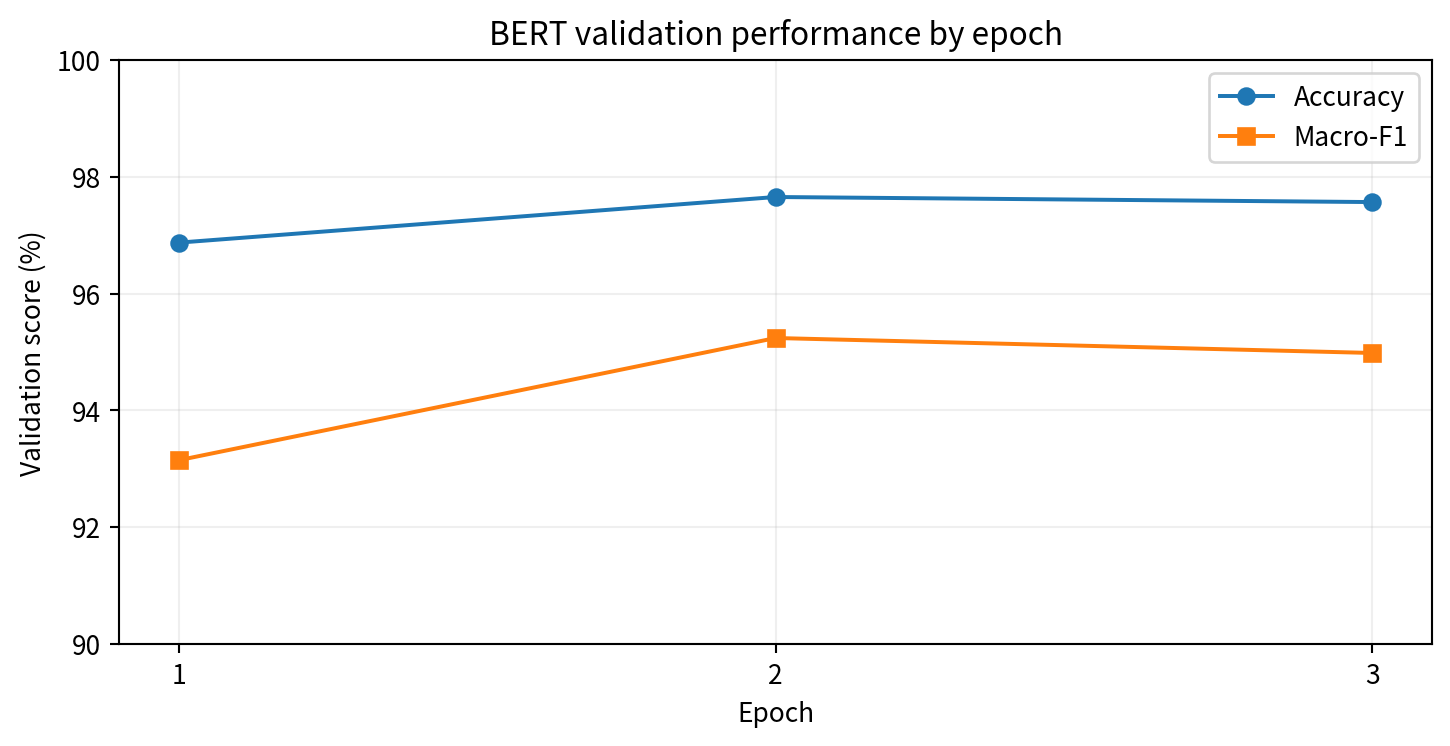
\includegraphics[width=.85\linewidth]{fig3_bert_training.png}\caption{BERT 三轮训练的验证集指标变化}\end{figure}
第 2 轮的验证集 Accuracy 和 Macro-F1 均最高，第 3 轮略有下降。这说明继续训练并未稳定提升验证集性能。
\subsection{测试集结果}
BERT 最终测试集 Accuracy 为 0.9818，Macro-F1 为 0.9591。各类别结果如下：
\begin{table}[H]\centering\caption{BERT 测试集分类报告}\begin{tabular}{lrrrr}\toprule 类别 & Precision & Recall & F1 & Support\\\midrule business & 0.9200 & 0.9650 & 0.9420 & 143\\politics & 0.9638 & 0.9172 & 0.9399 & 145\\sports & 0.9954 & 0.9954 & 0.9954 & 864\\\bottomrule\end{tabular}\end{table}
BERT 的测试集 Accuracy 达到 98.18\%，Macro-F1 达到 95.91\%，我们使用预训练语言模型也能够有效完成当前新闻分类任务。

但与 Task 1 的词频词袋模型相比，BERT 的两个指标均略低。可能是因为当前数据集的类别能够通过关键词得到较好区分，同时BERT 最大序列长度限制为 64，可能截断部分文本信息。
\section{综合对比与讨论}
\begin{table}[H]\centering\caption{六种方法在 NYT 测试集上的结果}\begin{tabular}{lrr}\toprule 方法 & Accuracy & Macro-F1\\\midrule Binary BoW & 0.9887 & 0.9718\\Word Frequency BoW & \textbf{0.9896} & \textbf{0.9743}\\GloVe 100d & 0.9852 & 0.9646\\Word2Vec (AG News) & 0.9766 & 0.9416\\Word2Vec (NYT) & 0.9818 & 0.9542\\BERT & 0.9818 & 0.9591\\\bottomrule\end{tabular}\end{table}
\begin{figure}[H]\centering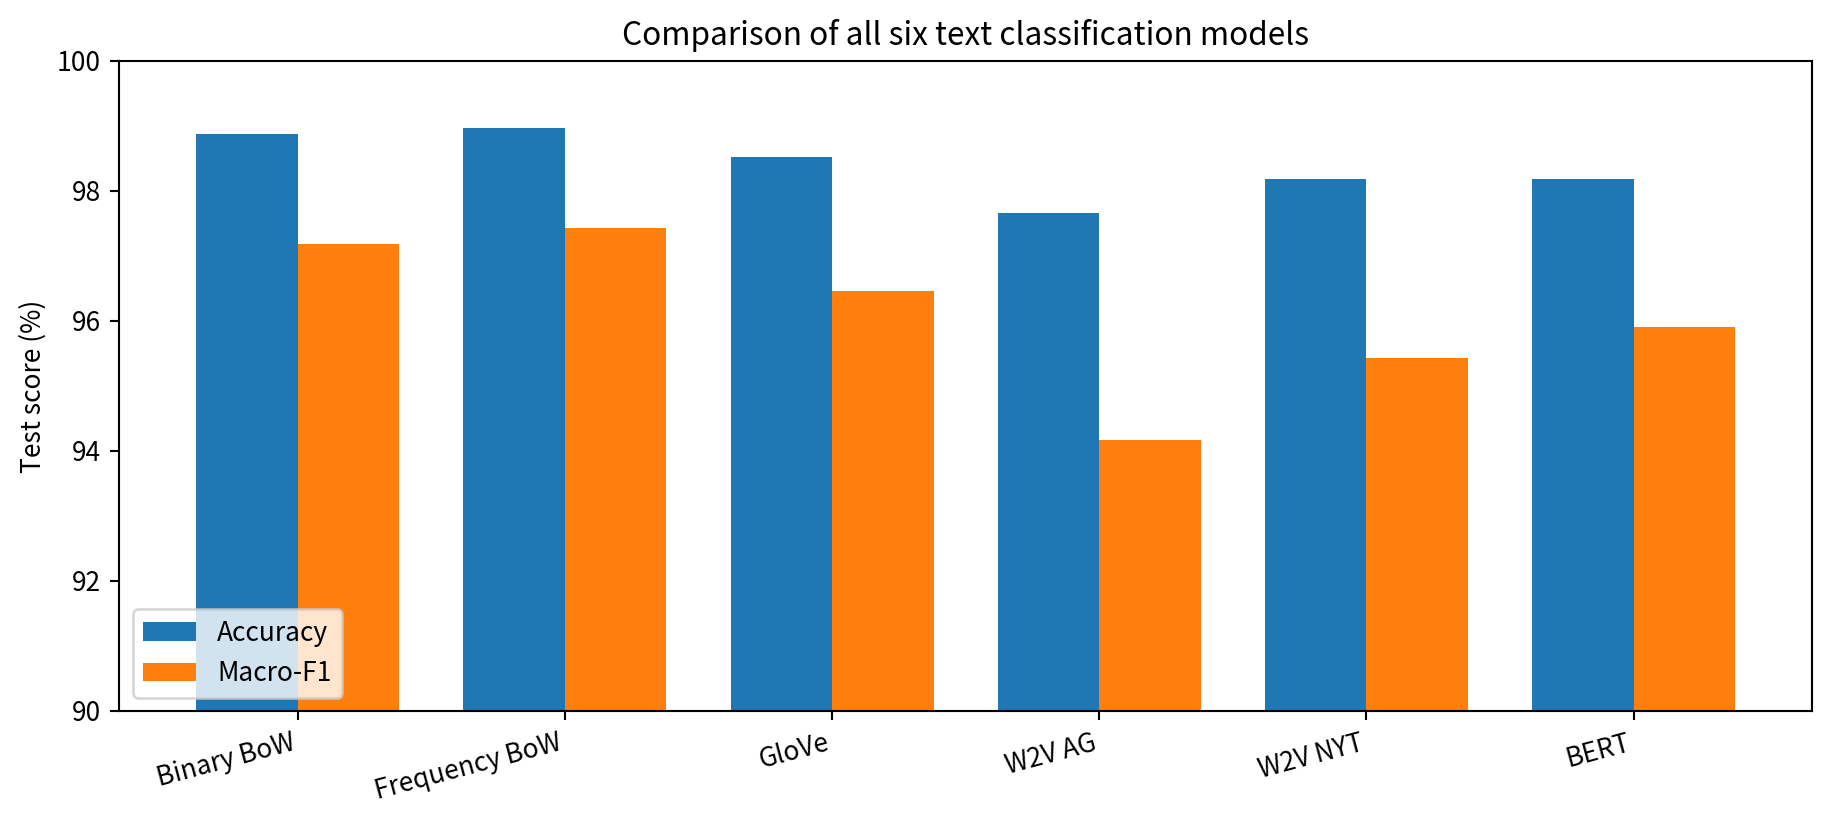
\includegraphics[width=\linewidth]{fig4_all_models.png}\caption{六种分类方法的测试集性能对比（纵轴从 90\% 起）}\end{figure}
六种方法均取得超过 97\% 的测试集 Accuracy。词频词袋结合逻辑回归整体表现最佳，说明当前数据集可能存在较强的词汇级类别区分信号。GloVe 在词向量方法中最好，BERT 虽具备上下文建模能力，但未超越词袋模型，可能与任务特征、64-token 截断限制及微调超参数有关。

值得注意的是，BERT 与 NYT Word2Vec 的 Accuracy 相同，但 Macro-F1 更高，说明相同总体准确率不代表各类别上的表现一致。对于当前体育类别占比较高的数据集，应结合两项指标评价模型。

\section{结论}
本实验完成了词袋、词向量与 BERT 三类文本分类方法的实现和比较。词频词袋在 NYT 测试集上获得最高 Accuracy（98.96\%）和 Macro-F1（97.43\%）；预训练 GloVe 优于两种自行训练的 Word2Vec；BERT 获得 98.18\% 的 Accuracy 和 95.91\% 的 Macro-F1。实验说明，模型复杂度与最终分类效果并不必然正相关，实际操作中要结合数据特点、训练资源与评价指标选择适合的文本表示方法。

\begin{thebibliography}{9}
\bibitem{mikolov} Mikolov, T., et al. Efficient Estimation of Word Representations in Vector Space. 2013.
\bibitem{glove} Pennington, J., Socher, R., Manning, C. D. GloVe: Global Vectors for Word Representation. EMNLP, 2014.
\bibitem{bert} Devlin, J., et al. BERT: Pre-training of Deep Bidirectional Transformers for Language Understanding. NAACL, 2019.
\bibitem{sklearn} Pedregosa, F., et al. Scikit-learn: Machine Learning in Python. JMLR, 2011.
\end{thebibliography}
\end{document}
